\documentclass{article}
\usepackage{algorithm}
\usepackage{algpseudocodex}
\usepackage{graphicx}
\usepackage{amsmath}
\usepackage{bm}
\title{CSEP501 : Compiler Construction: Homework 2}
\author{Karuna Sagar Krishna}

\begin{document}
    \maketitle

    \section*{Question 1}

    \subsection*{1a}
    The grammar is ambiguous since there are multiple leftmost/rightmost derivations for the same string as shown below for sentence $abab$.

    Following is 2 leftmost derivation of $abab$; notice the order in which the rules are applied is different:

    \begin{align*}
        S   & \rightarrow aSbS      && \textit{using S ::= aSbS} \\
            & \rightarrow abSaSbS   && \textit{using S ::= bSaS} \\
            & \rightarrow abaSbS    && \textit{using S ::= $\epsilon$} \\
            & \rightarrow ababS     && \textit{using S ::= $\epsilon$} \\
            & \rightarrow abab      && \textit{using S ::= $\epsilon$} \\
    \end{align*}

    \begin{align*}
        S   & \rightarrow aSbS      && \textit{using S ::= aSbS} \\
            & \rightarrow abS       && \textit{using S ::= $\epsilon$} \\
            & \rightarrow abaSbS    && \textit{using S ::= aSbS} \\
            & \rightarrow ababS     && \textit{using S ::= $\epsilon$} \\
            & \rightarrow abab      && \textit{using S ::= $\epsilon$} \\
    \end{align*}

    \subsection*{1b}
    Following is 2 rightmost derivation of $abab$; notice the order in which the rules are applied is different:

    \begin{align*}
        S   & \rightarrow aSbS      && \textit{using S ::= aSbS} \\
            & \rightarrow aSbaSbS   && \textit{using S ::= aSbS} \\
            & \rightarrow aSbaSb    && \textit{using S ::= $\epsilon$} \\
            & \rightarrow aSbab     && \textit{using S ::= $\epsilon$} \\
            & \rightarrow abab      && \textit{using S ::= $\epsilon$} \\
    \end{align*}

    \begin{align*}
        S   & \rightarrow aSbS      && \textit{using S ::= aSbS} \\
            & \rightarrow aSb       && \textit{using S ::= $\epsilon$} \\
            & \rightarrow abSaSb    && \textit{using S ::= bSaS} \\
            & \rightarrow abSab     && \textit{using S ::= $\epsilon$} \\
            & \rightarrow abab      && \textit{using S ::= $\epsilon$} \\
    \end{align*}

    \subsection*{1c}
    Following is the parse tree for the above derivations in order:

    Leftmost derivations:
    \begin{figure}[H]
        \centering
        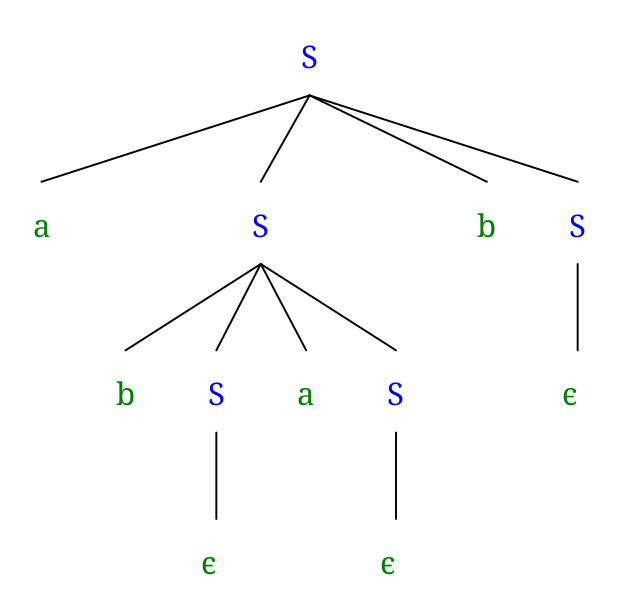
\includegraphics[width=.7\textwidth]{hw2-1c1.png}
    \end{figure}

    \begin{figure}[H]
        \centering
        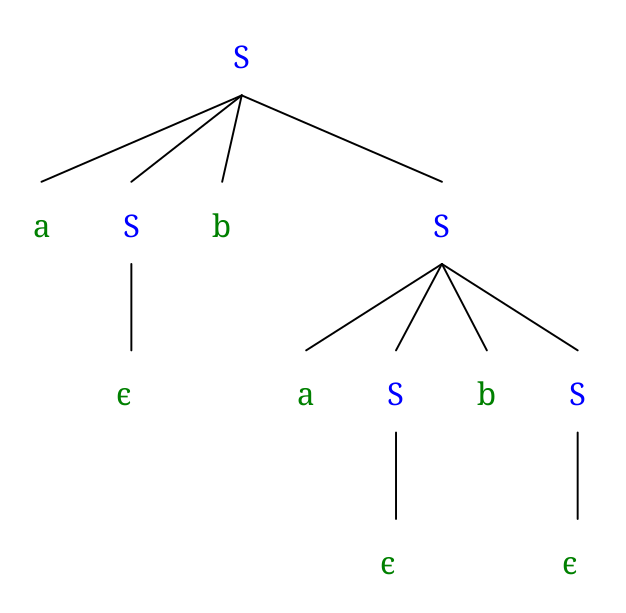
\includegraphics[width=.7\textwidth]{hw2-1c2.png}
    \end{figure}

    Rightmost derivations:
    \begin{figure}[H]
        \centering
        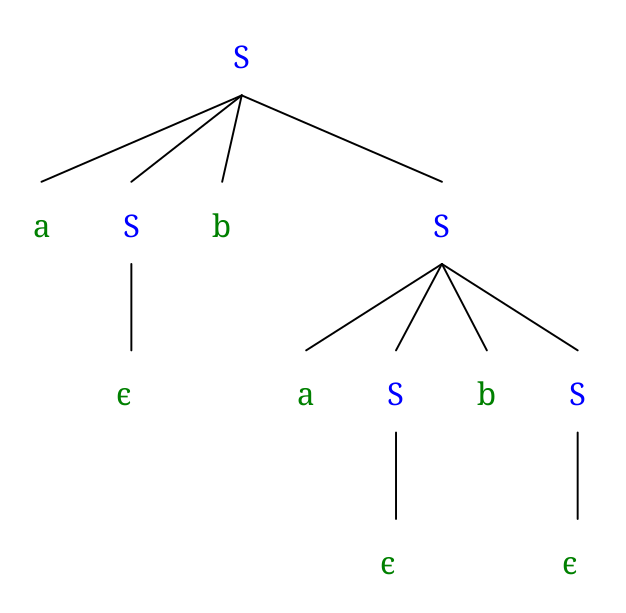
\includegraphics[width=.7\textwidth]{hw2-1c3.png}
    \end{figure}

    \begin{figure}[H]
        \centering
        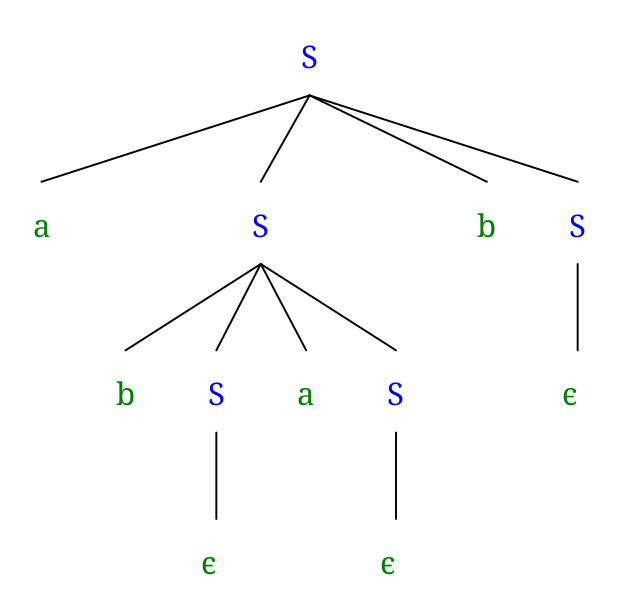
\includegraphics[width=.7\textwidth]{hw2-1c4.png}
    \end{figure}

    \section*{Question 2}

    \subsection*{2a}
    The leftmost derivation of $(x,(x,x))$ is:

    \begin{align*}
        S   & \rightarrow (L)       && \textit{using S ::= (L)} \\
            & \rightarrow (L,S)     && \textit{using L ::= L,S} \\
            & \rightarrow (S,S)     && \textit{using L ::= S} \\
            & \rightarrow (x,S)     && \textit{using S ::= x} \\
            & \rightarrow (x,(L))   && \textit{using S ::= (L)} \\
            & \rightarrow (x,(L,S)) && \textit{using L ::= L,S} \\
            & \rightarrow (x,(S,S)) && \textit{using L ::= S} \\
            & \rightarrow (x,(x,S)) && \textit{using S ::= x} \\
            & \rightarrow (x,(x,x)) && \textit{using S ::= x} \\
    \end{align*}

    \subsection*{2b}
    The rightmost derivation of $(x,(x,x))$ is:
    
    \begin{align*}
        S   & \rightarrow (L)       && \textit{using S ::= (L)} \\
            & \rightarrow (L,S)     && \textit{using L ::= L,S} \\
            & \rightarrow (L,(L))   && \textit{using S ::= (L)} \\
            & \rightarrow (L,(L,S)) && \textit{using L ::= L,S} \\
            & \rightarrow (L,(L,x)) && \textit{using S ::= x} \\
            & \rightarrow (L,(S,x)) && \textit{using L ::= S} \\
            & \rightarrow (L,(x,x)) && \textit{using S ::= x} \\
            & \rightarrow (S,(x,x)) && \textit{using L ::= S} \\
            & \rightarrow (x,(x,x)) && \textit{using S ::= x} \\
    \end{align*}

    \subsection*{2c}
    Since the LR1 parser discovers the rightmost derivation in reverse order, it makes sense to first find the rightmost derivation for the target sentence $(x,x,x)$. Using this rightmost derivation, we show the steps of the parser.

    The rightmost derivation of $(x,x,x)$ is:

    \begin{align*}
        S   & \rightarrow (L)       && \textit{using S ::= (L)} \\
            & \rightarrow (L,S)     && \textit{using L ::= L,S} \\
            & \rightarrow (L,x)     && \textit{using S ::= x} \\
            & \rightarrow (L,S,x)   && \textit{using L ::= L,S} \\
            & \rightarrow (L,x,x)   && \textit{using S ::= x} \\
            & \rightarrow (S,x,x)   && \textit{using L ::= S} \\
            & \rightarrow (x,x,x)   && \textit{using S ::= x} \\
    \end{align*}

    The steps of the LR1 parser are shown below. Bottom of the stack is represented by \$.

    \begin{center}
        \begin{tabular}{ l l c l r }
            \hline
            Iteration   &   Stack   &   Next Word   &   Action  &   Remaining Input \\
            \hline
            1       &   \$          &   (   &   shift   &   (x,x,x)  \\
            2       &   \$(         &   x   &   shift   &   x,x,x)   \\
            3       &   \$(x        &   ,   &   reduce  &   ,x,x)    \\
            4       &   \$(S        &   ,   &   reduce  &   ,x,x)    \\
            5       &   \$(L        &   ,   &   shift   &   ,x,x)    \\
            6       &   \$(L,       &   x   &   shift   &   x,x)     \\
            7       &   \$(L,x      &   ,   &   reduce  &   ,x)      \\
            8       &   \$(L,S      &   ,   &   reduce  &   ,x)      \\
            9       &   \$(L        &   ,   &   shift   &   ,x)      \\
            10      &   \$(L,       &   x   &   shift   &   x)       \\
            11      &   \$(L,x      &   )   &   reduce  &   )        \\
            12      &   \$(L,S      &   )   &   reduce  &   )        \\
            13      &   \$(L        &   )   &   shift   &   )        \\
            14      &   \$(L)       &   eof &   reduce  &   eof      \\
            15      &   \$S         &   eof &   accept  &   eof      \\
        \end{tabular}
    \end{center}

    \subsection*{2d}
    By using the right recursive production rule, it seems that the depth of the stack increases as shown below. The max depth in the example below is 7 while the max depth when using left recursive production rule is 4. This makes sense because the right recursive rules forces us to push more words on the stack until we can recognize and reduce it.

    The rightmost derivation of $(x,x,x)$ is:

    \begin{align*}
        S   & \rightarrow (L)       && \textit{using S ::= (L)} \\
            & \rightarrow (S,L)     && \textit{using L ::= S,L} \\
            & \rightarrow (S,S,L)   && \textit{using L ::= S,L} \\
            & \rightarrow (S,S,S)   && \textit{using L ::= S} \\
            & \rightarrow (S,S,x)   && \textit{using S ::= x} \\
            & \rightarrow (S,x,x)   && \textit{using S ::= x} \\
            & \rightarrow (x,x,x)   && \textit{using S ::= x} \\
    \end{align*}

    The steps of the LR1 parser are shown below:

    \begin{center}
        \begin{tabular}{ l l c l r }
            \hline
            Iteration   &   Stack   &   Next Word   &   Action  &   Remaining Input \\
            \hline
            1       &   \$          &   (   &   shift   &   (x,x,x)  \\
            2       &   \$(         &   x   &   shift   &   x,x,x)   \\
            3       &   \$(x        &   ,   &   reduce  &   ,x,x)    \\
            4       &   \$(S        &   ,   &   shift   &   ,x,x)    \\
            5       &   \$(S,       &   x   &   shift   &   x,x)    \\
            6       &   \$(S,x      &   ,   &   reduce  &   ,x)     \\
            7       &   \$(S,S      &   ,   &   shift   &   ,x)      \\
            8       &   \$(S,S,     &   x   &   shift   &   x)      \\
            9       &   \$(S,S,x    &   )   &   reduce  &   )      \\
            10      &   \$(S,S,S    &   )   &   reduce  &   )       \\
            11      &   \$(S,S,L    &   )   &   reduce  &   )        \\
            12      &   \$(S,L      &   )   &   reduce  &   )        \\
            13      &   \$(L        &   )   &   shift   &   )        \\
            14      &   \$(L)       &   eof &   reduce  &   eof      \\
            15      &   \$S         &   eof &   accept  &   eof      \\
        \end{tabular}
    \end{center}
    
    \section*{Question 3}
    Note, I'm only defining the grammar rules that would necessary to generate the target sentence \textit{time flies like an arrow; fruit flies like a banana}.

    First, we define terminal tokens (syntactic categories; parts of speech) returned by the scanner:
    \begin{align*}
        v & - \textit{verb} \\
        p & - \textit{preposition} \\
        a & - \textit{article} \\
        n & - \textit{noun} \\
    \end{align*}

    Next, we have the following non-terminal tokens:
    \begin{align*}
        T & - \textit{sentence (target)} \\
        C & - \textit{clause} \\
        S & - \textit{subject} \\
        O & - \textit{object} \\
    \end{align*}

    Next, we define the production rules:
    \begin{align*}
        T   & ::= \textit{C } | \textit{ C;C} \\
        C   & ::= \textit{S v O} \\
        S   & ::= \textit{n } | \textit{ n n} \\
        O   & ::= \textit{p a n } | \textit{ a n} \\
    \end{align*}

    So, this gives us the grammar $G$ formed by the above non-terminals, terminals, production rules and start symbol ($T$).

    For the target sentence, we associate its words with the following parts of speech:
    \begin{align*}
        time    & - \textit{n or v} \\
        flies   & - \textit{n or v}\\
        like    & - \textit{n or v or p} \\
        an      & - \textit{a} \\
        arrow   & - \textit{n} \\
        fruit   & - \textit{n} \\
        a       & - \textit{a} \\
        banana  & - \textit{n} \\
    \end{align*}

    Note, each word of the sentence has multiple possible syntactic category that can be associated with it. This can cause confusion/challenge to the scanner and parser. Lets consider one possible leftmost derivation of the target sentence:
    \begin{align*}
        T   & \rightarrow \textit{C;C}               && \textit{using T ::= C;C}     \\
            & \rightarrow \textit{S v O;C}           && \textit{using C ::= S v O}   \\
            & \rightarrow \textit{n v O;C}           && \textit{using S ::= n}       \\
            & \rightarrow \textit{n v p a n;C}       && \textit{using O ::= p a n}   \\
            & \rightarrow \textit{n v p a n;S v O}   && \textit{using C ::= S v O}   \\
            & \rightarrow \textit{n v p a n;n v O}   && \textit{using S ::= n}       \\
            & \rightarrow \textit{n v p a n;n v p a n} && \textit{using O ::= p a n} \\
    \end{align*}

    \begin{figure}[H]
        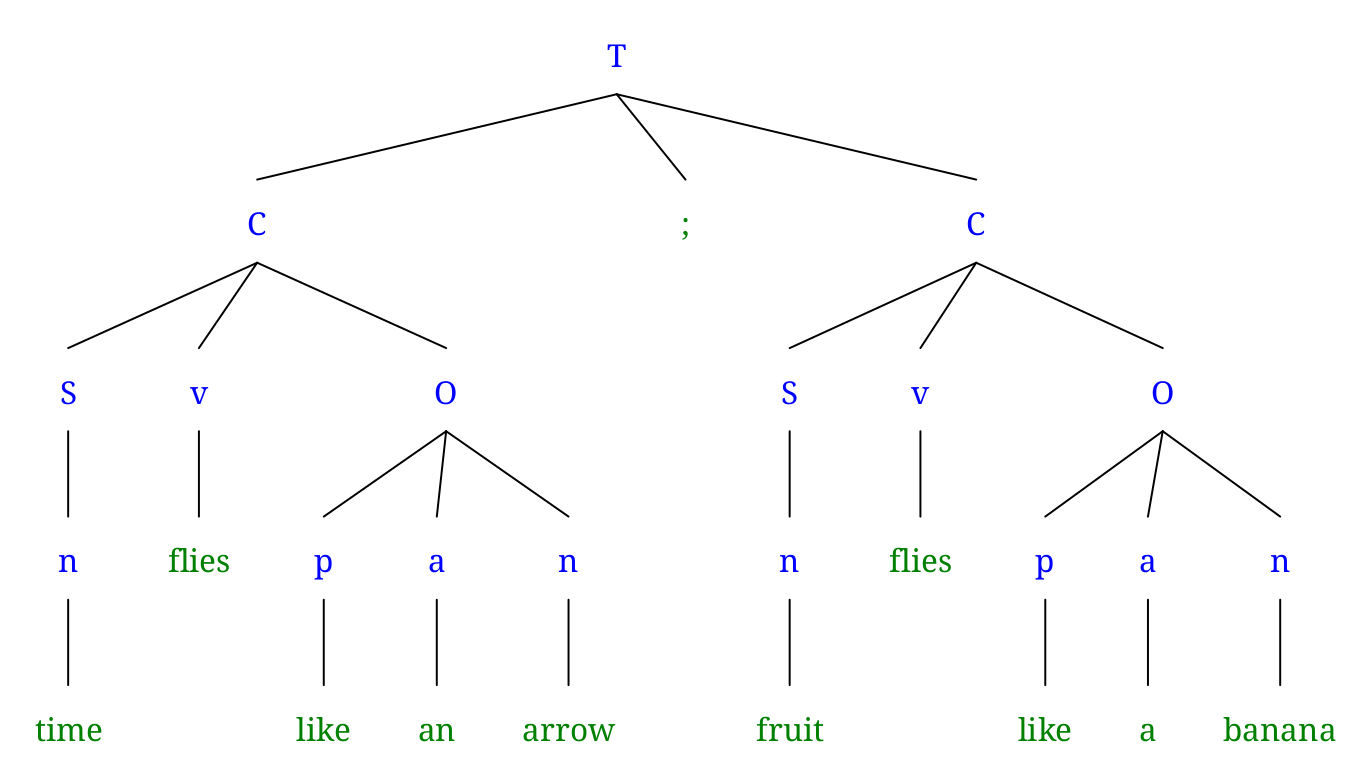
\includegraphics[width=1\textwidth]{hw2-3q1.png}
    \end{figure}

    So this derivation tells us that - time (noun) moves similar to an arrow. Then it goes on to say that - fruit (noun) also moves similar to a banana. The first part of the sentence makes sense since it indicates that time keeps progressing forward however, the second part of the sentence doesn't make sense since fruit cannot fly and neither can banana on its own.

    Consider another possible leftmost derivation of the target sentence:
    \begin{align*}
        T   & \rightarrow \textit{C;C}               && \textit{using T ::= C;C}     \\
            & \rightarrow \textit{S v O;C}           && \textit{using C ::= S v O}   \\
            & \rightarrow \textit{n v O;C}           && \textit{using S ::= n}       \\
            & \rightarrow \textit{n v p a n;C}       && \textit{using O ::= p a n}   \\
            & \rightarrow \textit{n v p a n;S v O}   && \textit{using C ::= S v O}   \\
            & \rightarrow \textit{n v p a n;n n v O} && \textit{using S ::= n n}   \\
            & \rightarrow \textit{n v p a n;n n v a n} && \textit{using O ::= a n} \\
    \end{align*}

    \begin{figure}[H]
        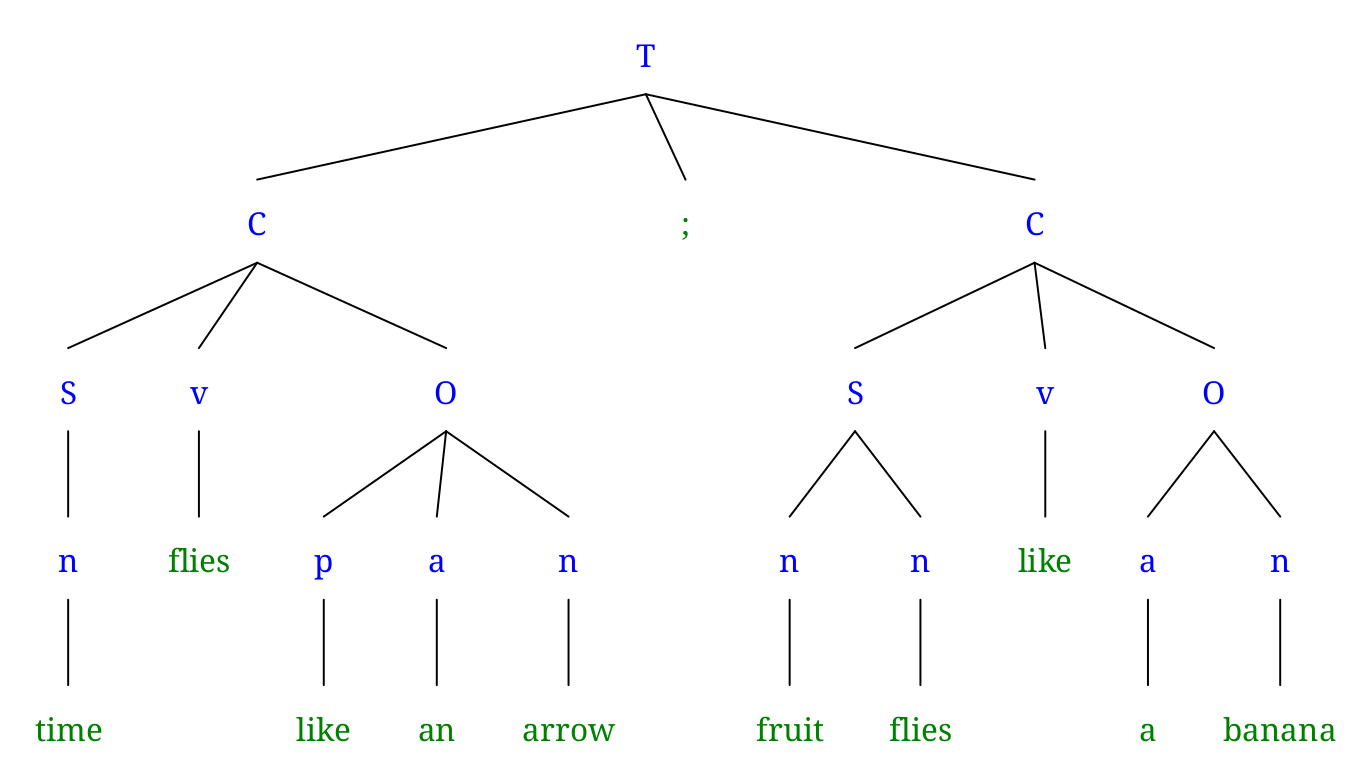
\includegraphics[width=1\textwidth]{hw2-3q2.png}
    \end{figure}

    The first clause has a similar derivation to the previous one i.e. time (noun) moves similar to an arrow. However, there is a change in the derivation for the second clause. It says that - a fruit fly (noun) is found of banana. This makes sense since fruit fly is an insect and its like to eat banana.

    This makes the grammar syntactically ambiguous since there are multiple leftmost derivations for the same target sentence. Further, it is also semantically ambiguous since the same sentence can have multiple meanings.
\end{document}
